\section{Fine State Machine}

\subsection{Zustandsbasierte Systeme}
Viele Embedded Systeme k\"onnen Zustandsbasiert implementiert werden und dabei ist kein Betriebssystem auf dem Controller notwendig.
\subsubsection{Asynchron vs.synchrone FSMs \buch{p.6}}
\begin{itemize}
  \item Bei (elektronisch implementierten) asynchronen FSMs führen geänderte
  Inputsignale direkt zu Zustandsänderungen. Sie sind deshalb "`schneller"',
  jedoch äusserst empfindlich auf Glitches und kaum tastbar.
  \item Bei synchronen FSMs werden die Inputsignale nur zu diskreten Zeitpunkten
  betrachtet, diese Systeme sind getaktet.
  \item Softwareimplementationen sind eigentlich immer synchron, da die Rechner
  getaktet sind. Wenn die Inputsignale mittels Interrupts behandelt werden, ist
  darauf zu achten, dass die Interrupts nicht fälschlicherweise gesetzt werden (
  ist Aufgabe der Elektronik)
  \item Rein softwareseitig besteht die Problematik der Asynchronizität nicht
\end{itemize}

\subsubsection{State-Event-Diagram \buch{p.8}}
\begin{itemize}
  \item Die Zustände werden mit einem Kreis gekennzeichnet
  \item Die Ereignisse werden mit Pfeilen zwischen den Zuständen bezeichnet
  (Transitionen)
  \item Die Aktionen werden entweder bei den Zuständen geschrieben oder bei den
  Transitionen (je nach Automatentyp)
  \item Die Ausführung einer Transition benötigt keine Zeit. Deshalb sind bei
  der Modellierung oft Zwischenzustände vorzusehen, z.B. "`Closing"', "`Starting
  up"', "`Booting"', etc.
\end{itemize}

\subsubsection{Mealy-Automat \buch{p.9}}
\begin{itemize}
  \item Der nächste Zustand $Z_{n+1}$ ist abhängig vom Input X und von $Z_n$:
  $Z_{n+1}=f(Z_n,X)$
  \item Der Output Y ist abhängig vom inneren Zustand $Z_n$ \textbf{und vom
  Input X}: $Y=g(Z_n, X)$
  \item Die Actions liegen deshalb bei den Transitionen
\end{itemize}

\subsubsection{Moor-Automat \buch{p.10}}
\begin{itemize}
  \item Der nächste Zustand $Z_{n+1}$ ist abhängig vom Input X und von $Z_n$:
  $Z_{n+1}=f(Z_n,X)$
  \item Der Output Y ist \textbf{nur} abhängig vom inneren Zustand $Z_n$: $Y=g(Z_n)$
  \item Die Actions liegen deshalb bei den Zuständen
\end{itemize}

\subsubsection{Zustandstabelle \buch{p.17}}

\begin{tabular}{|l|l|l|l|}
\hline
\textbf{Momentaner Zustand}&\textbf{Ereignis}&\textbf{Nächster
Zustand}&\textbf{Aktionen}\\
\hline
AUS&EIN-Taste&Hochlaufen&Motor ausschalten\\
&&&Kühlung ausschalten\\&&&Grüne Lampe aus\\&&&Rote Lampe aus\\
\hline
Hochlaufen&Drehzahl\_erreicht&Drehzahl\_ok&Motor einschalten\\
&Signal&&Kühlung einschalten\\ \cline{2-3}
&Aus-Taste&AUS&\\\cline{2-3}
&Wasserkühlung&Störung&\\
&Störung&&\\
\hline
Drehzahl\_ok&Wasserkühlung&Störung&Grüne Lampe anz.\\
&Störung&&\\ \cline{2-3}
&AUS-Taste&AUS&\\
\hline
Störung&RESET-Taste&AUS&Motor ausschalten\\
&&&Kühlung ausschalten\\&&&Rote Lampe anz.\\
\hline
\end{tabular}

\subsubsection{Nachteile von Zustandsdiagrammen \buch{p.19}}
\begin{itemize}
  \item Für einen Resetzustand muss von jedem State zum Resetstate eine Transition gezeichnet werden.
  \item Da Zustandsdiagramme flach sind (es gibt keine Hierarchie), werden sie bei
        praktisch relevanten Aufgaben schnell unübersichtlich
  \item In Zustandsdiagrammen kann keine zeitliche Parallelität modelliert werden
\end{itemize}

\begin{figure}[h]
  \centering
  {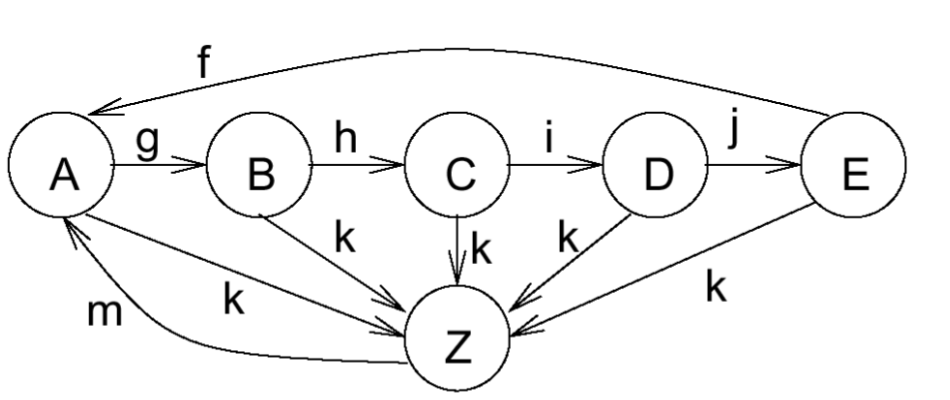
\includegraphics[width = 10cm]{images/FSM/reset_state}
  \caption{Nachteile bei einem Resetzustand}
  \label{fig:nachteile_reset_state}}
\end{figure}


\newcommand{\kreis}[1]{\unitlength1ex\begin{picture}(2.5,2.5)%
\put(0.75,0.75){\circle{3.5}}\put(0.75,0.75){\makebox(0,0){#1}}\end{picture}}

\subsection{Statecharts von Harel \buch{p.18}}
\subsubsection{Elemente der Statechart}
\begin{tabular}{ll}
$\bullet$&Anfangszustand (initial pseudo state)\\
$\diamond$& Entscheidung (choice)\\
$\bullet$& Kreuzung (junction)\\
$\times$& Terminator (terminate pseudo state)\\
\kreis{H}&flache Historie (shallow history): History-Mechanismus merkt sich
frühere Zustände\\
\kreis{H*}&tiefe Historie (deep history): Deep History-Mechanismus merkt sich
Zustände bis in die unterste Hierarchie\\
\kreis{}&Eintrittspunkt (entry point)\\
$\otimes$&Austrittspunkt (exit point)\\
\end{tabular}

\begin{figure}[h]
  \centering
  {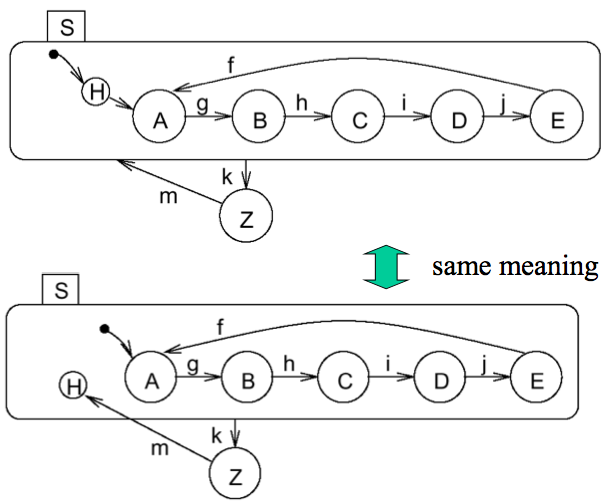
\includegraphics[scale = 0.3]{images/FSM/history_default_state_mechanism}  
  \caption{Combining history and default state mechanism}
  \label{fig:history_default_state_mechanism}}
\end{figure} 

\subsubsection{Definitonen\buch{p.22}}
\begin{itemize}
  \item Current states of FSMs are also called \textbf{active} states.
  \item States which are not composed of other states are called \textbf{basic
  states}.
  \item States containing other states are called \textbf{super-states}.
  \item for each basic state s, the super-states containing s are called
  \textbf{ancenstor states}.
  \item Super-states S are called \textbf{OR-super-states}, if exactly one of
  the sub-states of S is active whenever S is active.
\begin{figure}[h]
  \centering
  {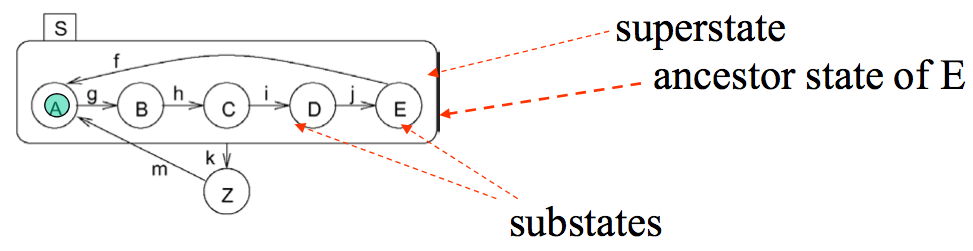
\includegraphics[scale = 0.3]{images/FSM/definition_statechart}  
  \caption{Definition Statechart}
  \label{fig:definition_statechart}}
\end{figure} 
\end{itemize}
\subsubsection{Parallälität (Concurrency)\buch{p.28}}
\begin{itemize}
  \item AND-super-states: Die FSM ist in allen sub-states einer super-state (siehe Abbildung \ref{fig:AND_super_state})
\end{itemize}
\begin{figure}[h]
  \centering
  {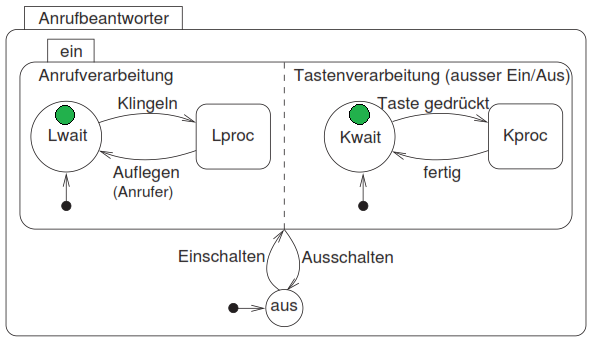
\includegraphics[scale = 0.4]{images/FSM/AND_super_state}  
  \caption{AND-super-state}
  \label{fig:AND_super_state}}
\end{figure} 

\subsubsection{Timers (nicht wait states)\buch{p.31}}
\begin{figure}[h]
  \centering
  {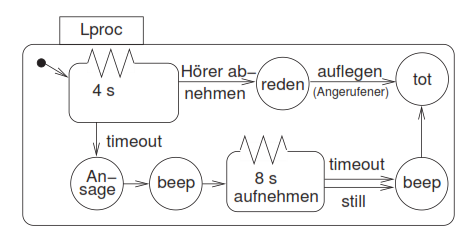
\includegraphics[scale = 0.2]{images/FSM/timer}  
  \caption{Using timers in an  answering machine}
  \label{fig:timer}}
\end{figure} 

\subsubsection{Vergleiche \buch{p.33}}
Statecharts im "`Lehrbuch der Objektmodellierung"':
\begin{itemize}
  \item LE4: pp87-95
  \item LE8: pp 197-205
  \item LE13: pp 339-348
\end{itemize}
\newpage
